\documentclass[11pt]{article}

\usepackage{homeworkpkg}
%% Local Macros and packages: add any of your own definitions here.
\usepackage{tikz}
\def\layersep{2.5cm}
\begin{document}

% Homework number, your name and NetID, and optionally, the names/NetIDs of anyone you collaborated with. If you did not collaborate with anybody, leave the last parameter empty.
\homework
    {3}
    {Lanxiao Bai (lbai5)}
    {}

\section*{Problem 1}
\textbf{Solution:} 
	Suppose the output of the first hidden layer is $\mathbf{h}$, then
	
	\begin{figure}[h]
        \begin{center}
        	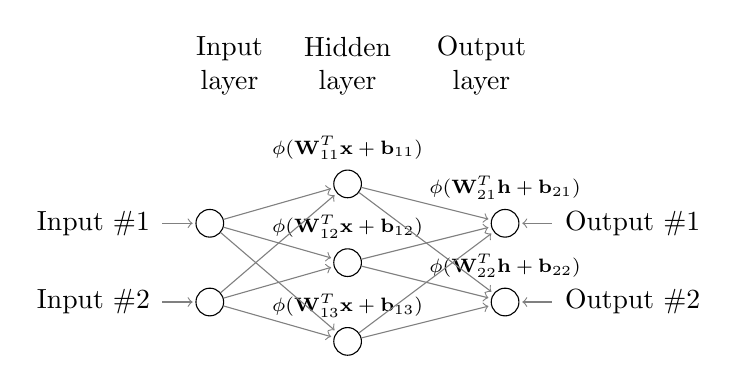
\begin{tikzpicture}[shorten >=1pt,->,draw=black!50, node distance=\layersep, every label/.append style={text=black, font=\scriptsize}]
    \tikzstyle{every pin edge}=[<-,shorten <=1pt]
    \tikzstyle{neuron}=[circle,fill=black!25,minimum size=10pt,inner sep=0pt]
    \tikzstyle{input neuron}=[neuron, draw=black, fill=white];
    \tikzstyle{output neuron}=[neuron, draw=black, fill=white];
    \tikzstyle{hidden neuron}=[neuron, draw=black, fill=white];
    \tikzstyle{annot} = [text width=4em, text centered]
        
    % Draw the input layer nodes
    \foreach \name / \y in {1,...,2}
        \node[input neuron, pin=left:Input \#\y] (H1-\name) at (0.5*\layersep,-\y) {};

    % Draw the hidden layer nodes
    \foreach \name / \y in {1,...,3}
        \path[yshift=0.5cm]
            node[hidden neuron, label=above:$\phi(\mathbf{W}_{1\y}^T\mathbf{x} + \mathbf{b}_{1\y})$] (H2-\name) at (1.2*\layersep,-\y cm) {};

    % Draw the output layer node
    \foreach \name / \y in {1,...,2}
    	\node[output neuron, label=above:$\phi(\mathbf{W}_{2\y}^T\mathbf{h} + \mathbf{b}_{2\y})$, pin=right:Output \#\y, right of=H1-\y] (O-\name) at (\layersep,-\y cm) {};

    % Connect every node in the input layer with every node in the
    % hidden layer.
    \foreach \source in {1,...,2}
        \foreach \dest in {1,...,3}
            \path (H1-\source) edge (H2-\dest);

    % Connect every node in the hidden layer with the output layer
    \foreach \source in {1,...,3}
    	\foreach \dest in {1,...,2}
        	\path (H2-\source) edge (O-\dest);

    % Annotate the layers
    \node[annot,above of=H2-1, node distance=1.5cm] (hl) {Hidden layer};
    \node[annot,left of=hl, node distance=1.5cm] {Input layer};
    \node[annot,right of=hl, node distance=1.7cm] {Output layer};
\end{tikzpicture}
		\caption{Neural Network when D = 2, H = 3, K = 2}
        \end{center}
    \end{figure}
\section*{Problem 2}
\textbf{Solution:} 
\begin{figure}[h]
        \begin{center}
        	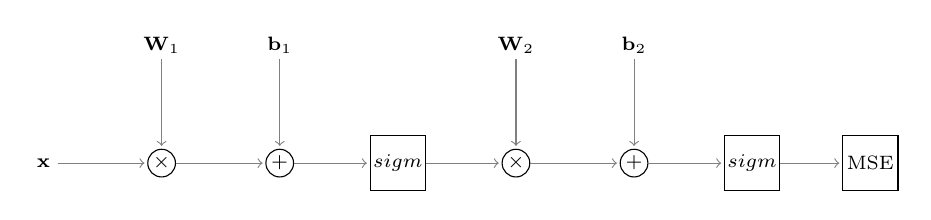
\begin{tikzpicture}[shorten >=1pt,->,draw=black!50, node distance=\layersep, every label/.append style={text=black, font=\scriptsize}]
    \tikzstyle{every pin edge}=[<-,shorten <=1pt]
    \tikzstyle{neuron}=[circle,fill=black!25,minimum size=10pt,inner sep=0pt, node distance=1.5cm]
    \tikzstyle{input neuron}=[neuron, draw=black, fill=white];
    \tikzstyle{output neuron}=[neuron, draw=black, fill=white];
    \tikzstyle{hidden neuron}=[neuron, draw=black, fill=white];
	\tikzstyle{loss}=[neuron, rectangle, draw=black, fill=white];
	\tikzstyle{activation}=[neuron, rectangle, draw=black, fill=white, minimum size=20pt];
	\tikzstyle{var}=[neuron, draw=white, fill=white];

    \node[var, label=center:$\mathbf{x}$] (x) {};
        
    % Draw the input layer nodes
    \node[input neuron, label=center:$\times$, right of=x, node distance=1.5cm] (H1-Prod) {};
    \node[var, label=center:$\mathbf{W}_1$, above of=H1-Prod, node distance=1.5cm] (W1) {};
    \node[hidden neuron, label=center:$+$, right of=H1-Prod, node distance=1.5cm] (H1-Sum){};
	\node[var, label=center:$\mathbf{b}_1$, above of=H1-Sum, node distance=1.5cm] (b1) {};
	\node[activation, label=center:$sigm$, right of=H1-Sum, node distance=1.5cm] (H1-Sigmoid) {};
    % Draw the hidden layer nodes
    \node[hidden neuron, label=center:$\times$, right of=H1-Sigmoid] (H2-Prod) {};
    \node[var, label=center:$\mathbf{W}_2$, above of=H2-Prod, node distance=1.5cm] (W2) {};
    \node[hidden neuron, label=center:$+$, right of=H2-Prod] (H2-Sum) {};
    \node[var, label=center:$\mathbf{b}_2$, above of=H2-Sum, node distance=1.5cm] (b2) {};
    \node[activation, label=center:$sigm$, right of=H2-Sum, node distance=1.5cm] (H2-Sigmoid) {};
    % Draw the output layer node
    
    \node[loss, minimum size=20pt, label=center:MSE, right of=H2-Sigmoid] (Loss) {};

    % Connect every node in the input layer with every node in the

    \path (x) edge (H1-Prod);
    \path (W1) edge (H1-Prod);
    \path (H1-Prod) edge (H1-Sum);
    \path (b1) edge (H1-Sum);
    \path (H1-Sum) edge (H1-Sigmoid);
    \path (H1-Sigmoid) edge (H2-Prod);
    \path (W2) edge (H2-Prod);
    \path (H2-Prod) edge (H2-Sum);
    \path (b2) edge (H2-Sum);
    \path (H2-Sum) edge (H2-Sigmoid);
    \path (H2-Sigmoid) edge (Loss);

\end{tikzpicture}
		\caption{Computational Graph of Neural Network when D = 2, H = 3, K = 2}
        \end{center}
    \end{figure}
    
    
\section*{Problem 3}
\textbf{Solution:} 
\[f(\mathbf{x_i}) = \phi(\mathbf{W}_2^T\phi(\mathbf{x}_i\mathbf{W}_1 + \mathbf{b}_1) + \mathbf{b}_2)\]

in which $\mathbf{W}_1$ is a $d \times H$ matrix, $\mathbf{W}_2$ is a $H \times K$ matrix, $\mathbf{b}_1$ is a $1 \times H$ matrix, $\mathbf{b}_1$ is a $1 \times K$ matrix and $\phi$ is an element-wise sigmoid function.
\section*{Problem 4}
\textbf{Solution:} 
	To make this clear, we first break down the formula into the following
	\begin{itemize}
		\item $l_{i} = \sum_{j = 1}^d w_{1_{ji}}x_{j} + b_{1_{i}}$
		\item $z_{i} = \phi(l_i)$
		\item $l'_{i} = \sum_{j = 1}^H w_{1_{ji}}z_{j} + b_{1_{i}}$
		\item $o_{i} = \phi(l'_{i})$
		\item $E = \frac{1}{2}\sum_{i = 1}^K(y_i - o_i)^2$
	\end{itemize}
	
	then we have 
	
	\begin{align}
		&\frac{\partial E}{\partial w_{hk}} = \frac{\partial E}{\partial o_k}\frac{\partial o_k}{\partial l'_k}\frac{\partial l'_k}{\partial w_{2_{hk}}}\nonumber\\
		&\phantom{\frac{\partial E}{\partial w_{hk}}} = \frac{\partial E}{\partial o_k}\frac{\partial o_k}{\partial l'_k}\frac{\partial l'_k}{\partial w_{hk}}\nonumber\\
		&\phantom{\frac{\partial E}{\partial w_{hk}}} = - (y_k - o_k)o_k(1 - o_k)z_{h}\nonumber
	\end{align}
	
	and 
	
	\begin{align}
		&\frac{\partial E}{\partial b_{k}} = \frac{\partial E}{\partial o_k}\frac{\partial o_k}{\partial l'_k}\frac{\partial l'_k}{\partial b_{2_{k}}}\nonumber\\
		&\phantom{\frac{\partial E}{\partial b_{k}}} = \frac{\partial E}{\partial o_k}\frac{\partial o_k}{\partial l'_k}\frac{\partial l'_k}{\partial b_{k}}\nonumber\\
		&\phantom{\frac{\partial E}{\partial b_{k}}} = - (y_k - o_k)o_k(1 - o_k)\nonumber
	\end{align}
	
	in which $o_{k} = \phi(\sum_{j = 1}^H w_{2_{jk}}\phi(\sum_{n = 1}^d w_{1_{nj}}x_{n} + b_{1_{j}}) + b_{2_{k}})$ and $z_{i} = \phi(\sum_{j = 1}^d w_{1_{ji}}x_{j} + b_{1_{i}})$.
\section*{Problem 5}
\textbf{Solution:} Similarly,
	\begin{align}
		&\frac{\partial E}{\partial w_{dh}} = \frac{\partial E}{\partial o_k}\frac{\partial o_k}{\partial l'_k}\frac{\partial l'_k}{\partial z_h}\frac{\partial z_h}{\partial l_h}\frac{\partial l_h}{\partial w_{1_{dh}}}\nonumber\\
		&\phantom{\frac{\partial E}{\partial w_{dh}}} = \frac{\partial E}{\partial o_k}\frac{\partial o_k}{\partial l'_k}\frac{\partial l'_k}{\partial z_h}\frac{\partial z_h}{\partial l_h}\frac{\partial l_h}{\partial w_{dh}}\nonumber\\
		&\phantom{\frac{\partial E}{\partial w_{hk}}} = - \left[\sum_k(y_k - o_k)o_k(1 - o_k)w^{(2)}_{hk}\right][z_{h}(1 - z_{h})]x_i\nonumber
	\end{align}
	
	and 
	
	\begin{align}
		&\frac{\partial E}{\partial b_{h}} = \frac{\partial E}{\partial o_k}\frac{\partial o_k}{\partial l'_k}\frac{\partial l'_k}{\partial z_h}\frac{\partial z_h}{\partial l_h}\frac{\partial l_h}{\partial b_{1_h}}\nonumber\\
		&\phantom{\frac{\partial E}{\partial b_{h}}} = \frac{\partial E}{\partial o_k}\frac{\partial o_k}{\partial l'_k}\frac{\partial l'_k}{\partial z_h}\frac{\partial z_h}{\partial l_h}\frac{\partial l_h}{\partial b_{h}}\nonumber\\
		&\phantom{\frac{\partial E}{\partial w_{hk}}} = - \left[\sum_k (y_k - o_k)o_k(1 - o_k)w^{(2)}_{hk}\right][z_{h}(1 - z_{h})]\nonumber
	\end{align}
	
	in which $o_{k} = \phi(\sum_{j = 1}^H w_{2_{jk}}\phi(\sum_{n = 1}^d w_{1_{nj}}x_{n} + b_{1_{j}}) + b_{2_{k}})$ and $z_{i} = \phi(\sum_{j = 1}^d w_{1_{ji}}x_{j} + b_{1_{i}})$.
\section*{Problem 6}
\textbf{Solution:} If more hidden layers are added into the network, when updating weights of input-hidden layer, the calculation of gradient should take in more differential terms based on chain rule.
\newpage \nocite{*}
\bibliographystyle{ims}
\bibliography{citations}

\end{document}
